% \documentclass[12pt]{article}

%%v helpful MIT exam schema, see http://www-math.mit.edu/~psh/exam/examdoc.pdf
 \documentclass[9pt]{exam} 
% \qformat{\textbf{Question \thequestion}\quad \thepoints\hfill } % Large depth to make space}
 \renewcommand{\thesubpart}{(\roman{subpart})}
 \renewcommand{\subpartlabel}{\thesubpart}
 \footer{}{}{Page \thepage\ de \numpages}
\addpoints
\pointsinmargin
% \boxedpoints
%\renewcommand{\questionshook}{\setlength{\itemsep}{1cm}}
%\renewcommand{\partshook}{
%	\setlength{\itemsep}{0.5cm}
%    	\setlength{\leftmargin}{-10pt}%
%}

\usepackage{cmbright}

\pagestyle{empty} %for handouts
\addtolength{\jot}{2em} % this makes all formulae a bit more spaced vertically for handouts
\setlength{\parindent}{0pt} %we're not writing a novel
%\renewcommand{\arraystretch}{2} %makes tables taller, so easier to write in

\usepackage[fleqn]{amsmath}
\usepackage{amssymb} %standard classy maths symbols
\usepackage[a4paper, margin=1in]{geometry} %makes it easy to specify where to put stuff on the page

\usepackage{siunitx} %v handy way of getting SI units to typeset correctly...
\sisetup{locale = FR} %... and now it will use a comma for decimals

\usepackage[utf8]{inputenc}

% \usepackage[french]{babel} % frenchify everything (e.g. a Table becomes a Tableau)
%\usepackage{lmodern} % font with nicer French characters than standard
%\usepackage{textcomp} % and more help for special characters

\usepackage{tcolorbox} % basic but good package for boxes around text
\tcbset{colback=black!5!white}
\usepackage{color} % colours
%\newcommand{\fillin}{\color{black!1!white}} %makes the text disappear
%\definecolor{fillin}{rgb} {1.00,1.00,1.00}
%\renewcommand{\fillin}{\color{blue}} \definecolor{fillin}{rgb} {0.00,0.00,1.00} %makes the filling in text appear (in blue)

\usepackage{enumitem} % can change the labels on lists, items, enumerates

\usepackage{tikz, pgfplots} % interval diagrams, sets, etc.
\usetikzlibrary{calc,trees,positioning,arrows,fit,shapes}

\begin{document}

\textbf{Name:} \dotfill

\begin{center}
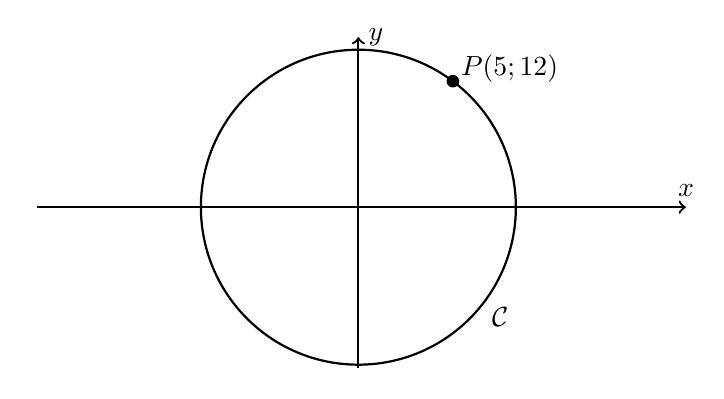
\begin{tikzpicture}[scale=0.4]
\clip (-10.5,-5.2) rectangle (10.7,5.7);
%\draw[help lines, step=1, white!50!gray] (-10.2,-5.6) grid (10.2,5.6);
%\draw[help lines,line width=.8pt,step=1] (-0.1,-0.1) grid (10.1,10.1);

\draw[thick, ->] (-10.2,0) -- (10.4,0) node[above] {$x$};
\draw[thick, ->] (0,-5.1) -- (0,5.4) node[right] {$y$};

%\foreach \x in {-10, -9, ..., 10}  \draw[thick] (\x,0.1) -- (\x,-0.1) node[below] {\scriptsize $\x$};
%\foreach \y in {-5, -4, ..., 5}  \draw[thick] (0.1,\y) -- (-0.1, \y) node[left] {\scriptsize $\y$};

\draw[thick] (0,0) circle (5);
\node at (4.5,-3.5) {$\mathcal{C}$};

\fill (3,4) circle(2mm);
\node at (4.8, 4.4) {$P(5;12)$};

\end{tikzpicture}
\end{center}

\begin{questions}

\question[3] Calculate the distance from the origin to $P(5; 12)$. \\
\emph{Points for the formula, substitution of values, and the result}
\fillwithdottedlines{28mm}

\question[2] What is the equation of the circle $\mathcal{C}$, centered on the origin, which goes through the point $P$?
\fillwithdottedlines{14mm}

\question[3] Calculate the gradient of $[OP]$.
\fillwithdottedlines{14mm}

\question[4] Determine the gradient-intercept form of the tangent to $\mathcal{C}$ passing through $P$.
\fillwithdottedlines{\stretch{1}}


\question[0] \textbf{Bonus.} Describe the curve $\mathcal{D}: x^2 + y^2 + 5y  = 12x$ and determine the intersections, if any, with $\mathcal{C}$.
\end{questions}

\begin{tcolorbox}

\textbf{Name of marker:}

\begin{center}
\gradetable[h][questions]
\end{center}

\end{tcolorbox}



\end{document}